\documentclass{bmd2010a}

\usepackage{subfig}

\begin{document}

\begin{flushleft}
{\fontsize{16pt}{20pt}\selectfont%
  Modeling Manually Controlled Bicycle Maneuvers\\}
\end{flushleft}

%%%%%%%%%%%%%%%% authors %%%%%%%%%%%%%%%
\begin{flushleft}
  {\fontsize{12}{14}{Ronald Hess, Jason K. Moore, Mont Hubbard and Dale L.
  Peterson}\\}
  \textit{Mechanical and Aerospace Engineering\\
          University of California, Davis\\
          One Shields Avenue, Davis, CA 95616, USA\\
          e-mail: rahess@ucdavis.edu, jkmoor@ucdavis.edu, mhubbard@ucdavis.edu,
          dlpeterson@ucdavis.edu
  }\vspace{10pt}\\
\end{flushleft}

\section*{Abstract}
An ability to predict the handling qualities of bicycles with different
physical characteristics remains an important research issue in the study of
manual control of single-track vehicles. Numerous factors affect bicycle
handling qualities as perceived by the rider, e.g. the dynamics of the bicycle
itself, the dynamics of the rider, the control characteristics of the rider,
and the manner in which the rider quantifies his/her opinion of the bicycle's
handling qualities. The work to be described follows in the footsteps
of~\cite{Lunteren1970} and \cite{Weir1972}, and utilizes a human operator model
discussed in~\cite{Hess2006} as applied to piloted aircraft control.
\begin{figure}[hb]
    \centering
    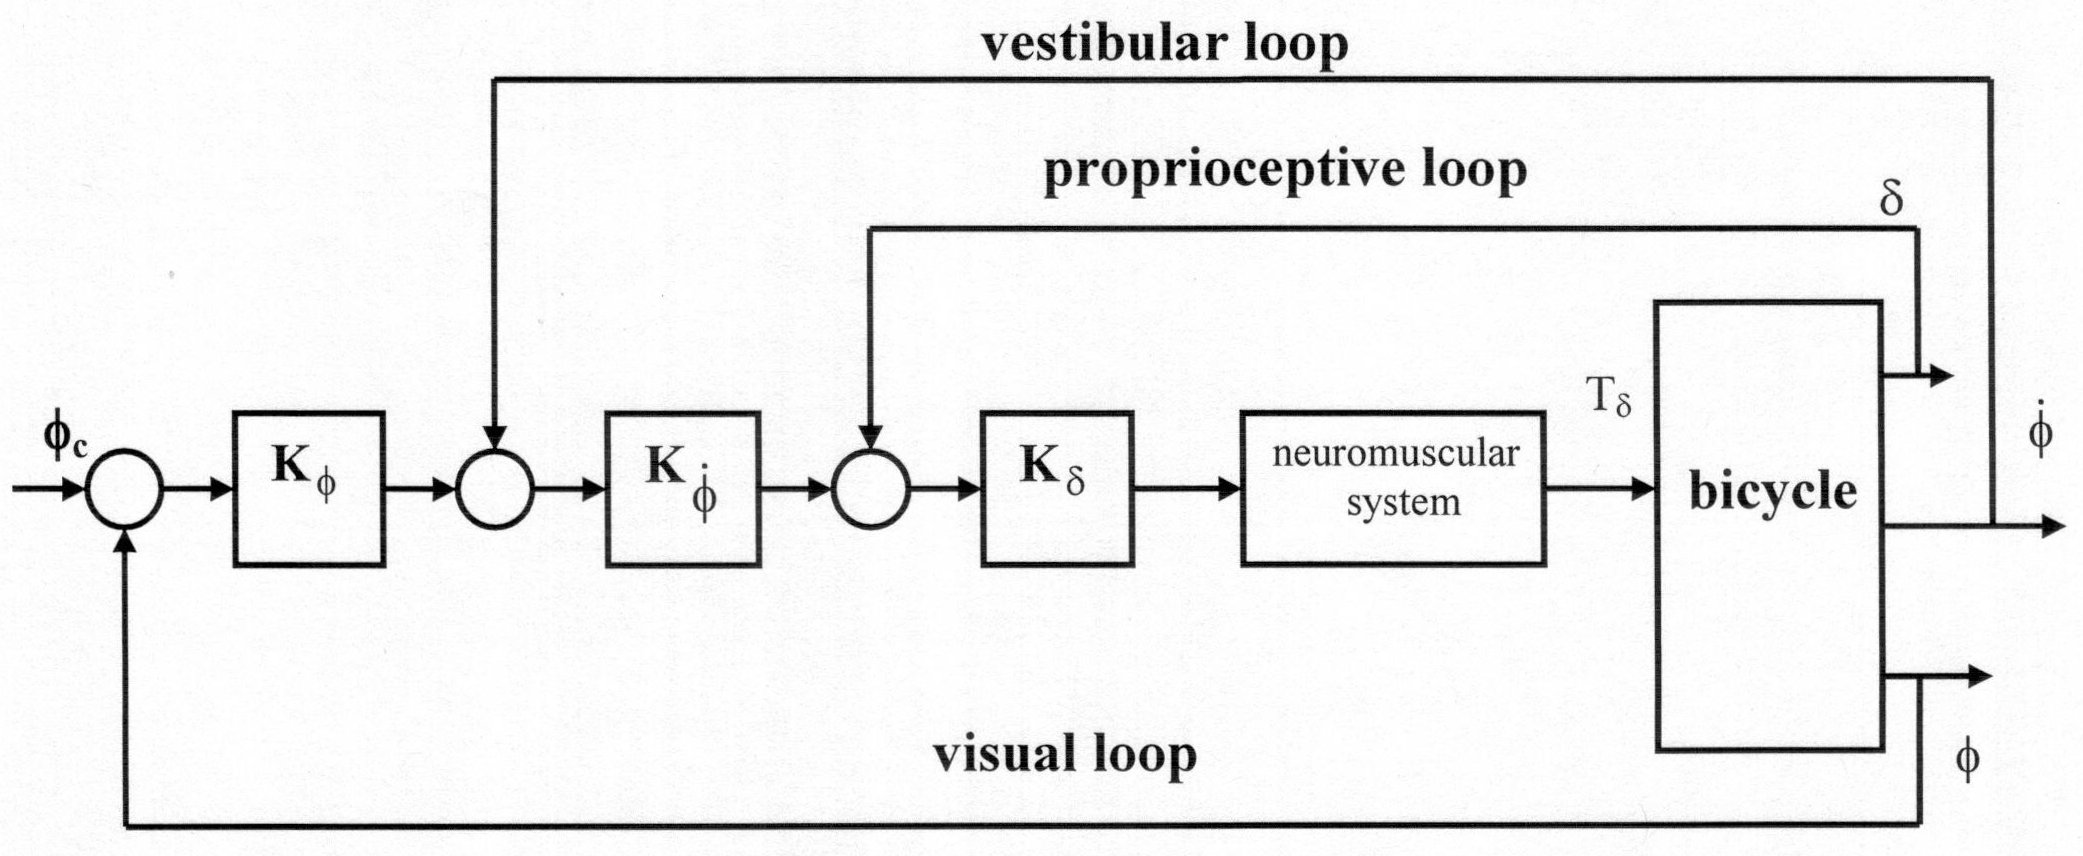
\includegraphics[width=0.65\columnwidth]{block.jpg}
    \caption{Block Diagram of Rider/Bicycle System}
    \label{fig:block}
\end{figure}

Figure~\ref{fig:block} is a block diagram representation of the
rider model for roll control of a bicycle, with appropriate sensory modalities
noted. As presented in Fig.~\ref{fig:block}, only three gains and a simple neuromuscular
system model parameterize the rider. By way of exposition in this brief
abstract, six bicycle models were chosen, five from existing bicycles as
parameterized by the second author in~\cite{Moore2010}, and the sixth being the ``benchmark'' bicycle from
~\cite{Meijaard2007}. All models are linear and valid for a forward velocity of 5 m/sec. A
simple two meter lane change and lane return maneuver was selected as a simple
task.
Figure~\ref{fig:path} shows the maneuver paths of the six rider/bicycles, where the bicycle
coordinate shown is associated with the rear wheel contact point. The complete
rider model includes two additional outer-loop closures not shown in
Fig.~\ref{fig:block} (heading and lateral deviation). In addition, a simple model of rider preview
is included~\cite{Hess2003a}. Figure~\ref{fig:steer} shows the rider steering inputs for the
task. Figure~\ref{fig:handling} shows the ``Handling Qualities Sensitivity
Functions'' (HQSFs) for each vehicle.
The magnitude of each of these functions has been shown to correlate well with
handling qualities ratings for aircraft flight control~\cite{Hess2006}. As an example here,
the two functions with the lowest magnitudes in the frequency range of
importance for manual control ($0<\omega<10$ rad/sec) are associated with the two
bicycle models that are either stable or marginally unstable (one root just
into the right-half plane). Finally, Fig.~\ref{fig:bode} shows Bode diagrams for the
rider/bicycle open-loop transfer function for each application, showing that
the rider model follows the dictates of the well-known ``crossover model'' of the
human operator~\cite{McRuer1974}, appropriate for the dynamics of the
bicycles in question. The final paper will include nine bicycle models and
maneuvers and a thorough discussion of applying the HQSF to the prediction of
bicycle handling qualities.
\begin{figure}[tb]
    \centering
    \subfloat[Lane Change Performance]{\label{fig:path}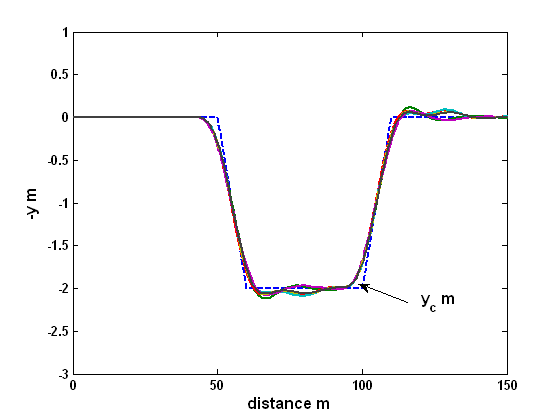
\includegraphics[width=0.38\columnwidth]{path.png}}
    \subfloat[Handling Qualities Sensitivity Functions]{\label{fig:handling}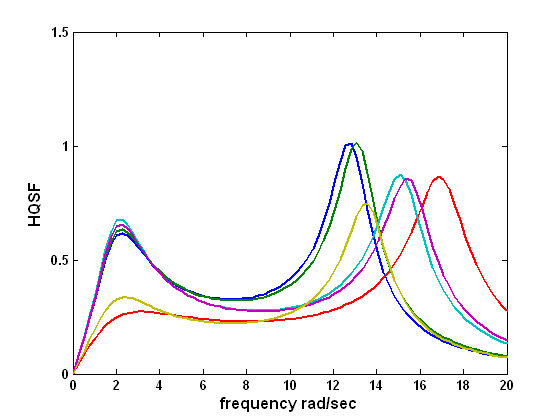
\includegraphics[width=0.38\columnwidth]{handling.png}}

    \subfloat[Rider Steering Inputs]{\label{fig:steer}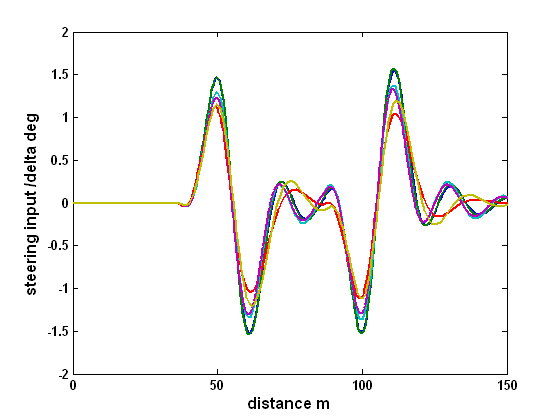
\includegraphics[width=0.38\columnwidth]{steer.png}}
    \subfloat[Bode Diagrams of Rider/Bicycle Open-Loop Transfer
    Functions]{\label{fig:bode}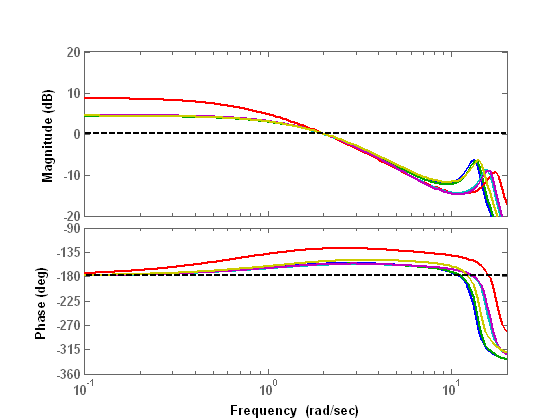
\includegraphics[width=0.38\columnwidth]{bode.png}}
    \caption{Linear simulation results and comparative metrics for six bicycles.}
    \label{fig:plots}
\end{figure}
\bibliographystyle{acm}
\bibliography{bicycle}
\end{document}
